\documentclass{article}

\usepackage{graphicx} % Required for inserting images
\usepackage{wrapfig}
\usepackage[table,xcdraw]{xcolor}
\usepackage{hyperref}
\usepackage[export]{adjustbox}
\usepackage{geometry}
\usepackage{listings}
\usepackage{caption}
\usepackage{subfigure}
\usepackage{tikz}
\usepackage{enumitem}
\usepackage{multirow}
\usepackage{forest}
\usepackage[bottom]{footmisc}
\usepackage{amsmath}
\usepackage{longtable}



\setcounter{secnumdepth}{4}
\setcounter{tocdepth}{4}
\geometry{a4paper,
 total={150mm,257mm},
 left=15mm,
 right=15mm,
 top=20mm}

 \begin{document}
  \tableofcontents

    
  \section{Crittografia Simmetrica}
    Se parliamo di crittografia Simmetrica, stiamo considerando uno schema in cui sono presenti almeno 2 agenti (Bob, Alice) che devono scambiare un messaggio in maniera sicura senza che un terzo (che potrebbe avere intenzioni malevole) possa capire il messaggio. 
    Il modello quindi prevede una funzione di cifrazione (Enc) e una funzione di decifrazione (Dec), una chiave condivisa (k) e due tipi di messaggio, \textit{x} detto messaggio in chiaro (plaintext) e \textit{y} detto messaggio cifrato (ciphertext) ; la funzione di criptazione è determinata da un algoritmo che pubblicamente conosciuto, quello che invece rende sicuro l'utilizzo della cifratura simmetrica è la segretezza e lunghezza della chiave. 
    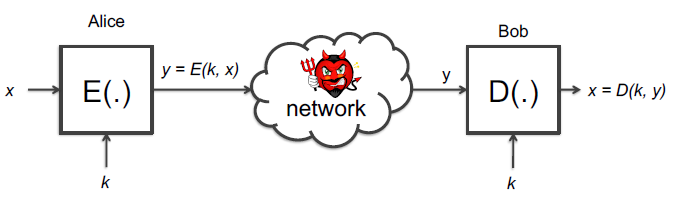
\includegraphics{./immagini/modello.png} 
    
    \paragraph{Definizione di Cifrario}
        Un cifrario, o schema di cifratura, è defito su una tripletta composta da (K,P,C) usata nelle funzioni di (Gen,Enc,Dec) definite con questi domini: 
         \begin{align}
            &Gen: Z^+ \to K funzione generatrice di chiavi\\  
            &Enc: P \times K \to C  funzione di cifratura\\
            &Dec : C \times K \to P funzione di decifratura\\
            &x \in P , y \in C , k \in K\\
            &y = Enc(k,x)\\
            &x = Dec(k,y)
        \end{align}
        \subparagraph{Proprieta di cifratura}
            La cifratura deve anche rispettare le seguenti proprieta: 
            \begin{description}
                 \item[Correttezza]: $\forall p \in P \land k \in K, \exists Dec(k,Enc(k,p)) = p$
                 \item[Sicurezza]:  Un cifrario simmetrico è sicuro $\iff \forall (p,c), p \in P \land c \in C  \Rightarrow$ 
                 \begin{itemize}
                            \item dato \textit{c} ciphertext, è "difficile" determinare \textit{p} plaintext senza conoscere la chiave \textit{k}, e viceversa
                            \item è "difficile" determinare \textit{k} chiave, ammenoche non sia stata già usata una volta
               \end{itemize}
            \end{description}

        \subparagraph{Esempio : Sostituzione monoalfabetca} 
            Vediamo quindi un tipo di cifratura a sostituzione, dove la chiave è la permutazione dell' alfabeto. L' algoritmo prevede la sostituzione delle lettere della parola con le corrispondenti dell' alfabeto shiftato, e per decriptare si usa l' algoritmo al contrario. Le chiavi quindi possono essere circa  26! cioè circa $4\cdot10^26$, quindi tentare un attacco a forza bruta non è possibile, ma è possibile applicare tecniche di Crittoanalisi analizzando alcune proprietà che riguardano i linguaggi come : la frequenza delle lettere, la generalizzazione delle coppie e triple di lettere, la frequenza delle parole corte se sono identificati i separatori.  
    \paragraph{Crittoanalisi}        
            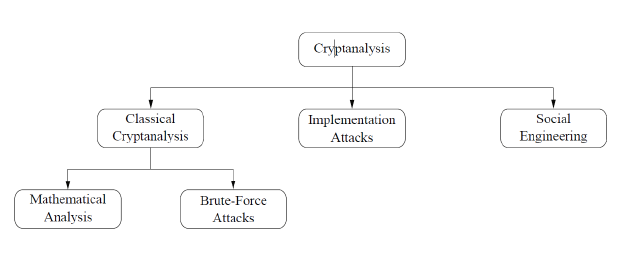
\includegraphics{./immagini/crittoanalisi.png}
               
          \subparagraph{Complessità dell'attacco} Viene definito da:
                \begin{description}
                    \item[Complessità dei Dati:] Numero previsto di unità dei dati in ingresso richiesti.
                    \item[Complessità di Storage:] Numero previsto delle unità di storage richiesti.
                    \item[Complessità di Elaborazione:] Numero previsto di operazioni richiesti per processare i dati in input o/e per riempire la memoria con dati.
                \end{description}
            
           \subparagraph{Tipi di attacco} Si possono classificare in:
               
                \begin{itemize}
                    \item Ciphertext-only attack
                    \item Known-plaintext attack
                    \item Chosen-plaintext attack (CPA)
                \end{itemize}
                Se un metodo è sicuro contro i CPA, allora è sicuro anche contro gli altri.
            \subparagraph{Principi di Kerchoff}

            \begin{description}
                \item[Massima di Kerckhoffs] Un sistema crittografico dovrebbe rimanere sicuro anche se tutto del sistema, tranne la chiave, è di pubblico dominio.
                
                \item[Massima di Shannon] Il nemico conosce il sistema.
                
                \item[Massima di Bruce Schneier] Meno e più semplici sono i segreti da custodire per garantire la sicurezza del sistema, più facile sarà mantenerne la sicurezza.
            \end{description}

            \textbf{Consigli per mantenera la sicurezza facile}
            \begin{itemize}
                \item Le chiavi sono piccoli segreti.
                \item Conservare piccoli segreti è più facile che conservare grandi segreti.
                \item Sostituire piccoli segreti, una volta eventualmente compromessi, è più facile (ed economico) che sostituire grandi segreti.
            \end{itemize}

        \paragraph{Esempi di cifrari} 
            \subparagraph{Cifrario di cesare}

            Siano $PT$, $CT$ e $K$ elementi dell'anello $Z_{26}$.

            \begin{itemize}
                \item \textbf{Cifratura (Encryption):} \[
                y = x + k \mod 26
                \]
                
                \item \textbf{Decifratura (Decryption):} \[
                x = y - k \mod 26
                \]
                
                \item \textbf{Esempio:}
                \begin{itemize}
                    \item Testo in chiaro (Plaintext, $x$): ``\texttt{ATTACK}'' $\Rightarrow$ \[x = (0, 19, 19, 0, 2, 10)\]
                    \item Chiave ($k$): \[k = 17\]
                    \item Testo cifrato (Ciphertext, $y$): \[
                    y = (0+17, 19+17, 19+17, 0+17, 2+17, 10+17) \mod 26 = (17, 10, 10, 17, 19, 1)
                    \]
                    \item Risultato: ``\texttt{RKKRTB}''
                \end{itemize}
            \end{itemize}

            \subparagraph{Cifrario Affine}

            \textbf{Definizione}

Siano $a, b, x, y \in Z_{26}$.

\begin{itemize}
    \item \textbf{Cifratura (Encryption):}
    \[
    y = a \cdot x + b \mod 26
    \]
    
    \item \textbf{Decifratura (Decryption):}
    \[
    x = a^{-1} \cdot (y - b) \mod 26
    \]
    
    \item La chiave è $k = (a, b)$, con $\gcd(a, 26) = 1$
    
    \item \textbf{Esempio:}
    \begin{itemize}
        \item Testo in chiaro (Plaintext): ``\texttt{ATTACK}'' $\Rightarrow (0, 19, 19, 0, 2, 10)$
        \item Chiave $k = (9, 13)$
        \item Cifratura:
        \[
        y = (9 \cdot x + 13) \mod 26
        \]
        \[
        y = (13, 2, 2, 13, 5, 25)
        \]
        \item Testo cifrato (Ciphertext): ``\texttt{NCCNFZ}''
    \end{itemize}
\end{itemize}

\textbf{Calcolo dello spazio delle chiavi}

Lo spazio delle chiavi si calcola come:
\[
\text{Spazio delle chiavi} = N_a \cdot N_b
\]

Dove:
\begin{itemize}
    \item $N_a$ è il numero di valori possibili di $a$ tali che $\gcd(a, 26) = 1$. \\
    In questo caso: $N_a = 12$
    \item $N_b$ è il numero dei possibili valori di shift $b$ in $Z_{26}$. \\
    Quindi: $N_b = 26$
\end{itemize}

Pertanto, lo spazio delle chiavi è:
\[
12 \cdot 26 = 312
\]

\paragraph{Teorema di Shannon}

\subparagraph{Teorema di Shannon}
\begin{itemize}
    \item In un cifrario perfetto, $|K| \geq |M|$
    \item Ovvero, il numero di chiavi non può essere inferiore al numero di messaggi
\end{itemize}

\subparagraph{Dimostrazione (per assurdo):}
\begin{enumerate}
    \item Supponiamo che $|K| < |M|$
    \item Deve valere $|C| \geq |M|$, altrimenti il cifrario non è invertibile
    \item Quindi, $|C| > |K|$
    \item Sia $m \in M$ tale che $\Pr[M = m] \neq 0$; si calcoli $c_i \leftarrow E(k_i, m)$ per ogni $k_i \in K$
    \item Per il punto (3), esiste almeno un $c$ tale che $c \neq c_i$ per ogni $k_i \in K$
    \item Allora $\Pr[M = m \mid C = c] = 0$, che è diverso da $\Pr[M = m]$, contraddicendo la definizione di cifrario perfetto
\end{enumerate}

\subparagraph{Fatto.} Sia $\Pi = (\text{Gen}, \text{Enc}, \text{Dec})$ uno schema di cifratura con $|M| = |K| = |C|$. Lo schema è perfettamente sicuro se e solo se:
\begin{enumerate}
    \item  $\foreach k \in K$ è scelto con probabilità uniforme $1/|K|$ da Gen
    \item  $\foreach m \in M$ \land $c \in C \exist $k \in K$ tale che $E_k(m) = c$
\end{enumerate}

\subparagraph{Nota:}
\begin{itemize}
    \item La condizione 1 è facile da verificare
    \item La condizione 2 non richiede il calcolo di probabilità
\end{itemize}

\paragraph{Sicurezza incondizionata}
La perfetta segretezza è equivalente alla sicurezza incondizionata. In questo modello, si assume che un avversario disponga di risorse computazionali illimitate. L'osservazione del testo cifrato non fornisce quindi alcuna informazione utile all'avversario riguardo al messaggio originale.

\subparagraph{Condizioni necessarie}
\begin{itemize}
    \item I bit della chiave devono essere scelti in modo veramente casuale
    \item La lunghezza della chiave deve essere maggiore o uguale alla lunghezza del messaggio (secondo il teorema di Shannon)
\end{itemize}

            
 
       
        
    \end{document}